\documentclass[a4paper, 12pt]{article}

\usepackage[english]{babel}
\usepackage[utf8]{inputenc}
\usepackage[T1]{fontenc}
\usepackage{lmodern}
\usepackage{units}
\usepackage{eurosym}
\usepackage{amsmath}
\usepackage{amssymb}
\usepackage{amsthm}
\usepackage{amsfonts}
\usepackage{mathtools}
\usepackage{graphicx}
\usepackage{color}
%\usepackage{url}
\usepackage{hyperref}
\usepackage{enumerate}
\usepackage{enumitem}
\usepackage{pifont}
\usepackage{tikz-cd}
\usetikzlibrary{babel}
\usepackage{adjustbox}

% set margin and layout here
\usepackage[margin=0.5in]{geometry}

% commonly used math operators
\DeclareMathOperator{\diam}{diam}
\DeclareMathOperator{\rank}{rank}
\DeclareMathOperator{\im}{im}
\DeclareMathOperator{\Lin}{Lin}
\DeclareMathOperator{\Ann}{Ann}
\DeclareMathOperator{\Ass}{Ass}
\DeclareMathOperator{\Spec}{Spec}
\DeclareMathOperator{\mSpec}{mSpec}
\DeclareMathOperator{\Quot}{Quot}
\DeclareMathOperator{\Tor}{Tor}
\DeclareMathOperator{\Ext}{Ext}
\DeclareMathOperator{\coker}{coker}

% commonly used math objects
\newcommand{\D}{\mathbb{D}}
\renewcommand{\S}{\mathbb{S}}
\newcommand{\B}{\mathbb{B}}
\newcommand{\N}{\mathbb{N}}
\newcommand{\Z}{\mathbb{Z}}
\newcommand{\Q}{\mathbb{Q}}
\newcommand{\R}{\mathbb{R}}
\newcommand{\C}{\mathbb{C}}
\renewcommand{\P}{\mathbb{P}}

% commonly used math relations
\newcommand{\iso}{\cong}
\newcommand{\homeo}{\approx}
\newcommand{\htpeq}{\simeq}
\newcommand{\hlgeq}{\sim}
\newcommand{\idtfy}{\longleftrightarrow}

% commonly used math symbols
\newcommand{\closure}[1]{\overline{#1}}
\newcommand{\subideal}{\vartriangleleft}
\newcommand{\supideal}{\vartriangleright}

% title data - MODIFY
\title{Algebraic Topology 2 - Homework 1}
\author{Benjamin Benčina, 27192018}

\begin{document}

\maketitle

\underline{\textbf{Ex. 1:}}
Let $K$ be the Klein bottle.
\begin{enumerate}
	\item Let us calculate the $\Delta$-complex homology of $K$ with coefficients in $\Z$ and $\Z_m$ for all $m \geq 2$. First we focus on coefficients in $\Z$.
	We naturally start by looking at the fundamental rectangle of the Klein bottle. As seen in Figure \ref{fig:klein} (Hatcher, p. 102) below, we get two $2$-simplices $U$ and $L$, three $1$-simplices $a$, $b$ and $c$, and a single $0$-simplex denoted by $v$.
	\begin{figure}[h]
		\centering
		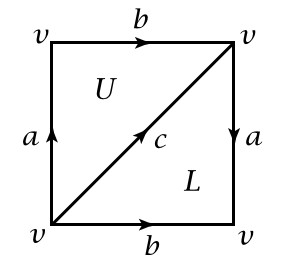
\includegraphics[scale=0.4]{klein.png}
		\label{fig:klein}
		\caption{Fundamental rectangle with $\Delta$-structure for Klein bottle}
	\end{figure}

	We obtain the following chain complex
	\[
	0 \to \Z(U, L) \to \Z(a, b, c) \to \Z(v) \to 0.
	\]
	Next we calculate the boundary maps. As there is merely one $0$-simplex, it is obvious that
	\[
	\partial_1 a = 0,\;
	\partial_1 b = 0,\;
	\partial_1 c = 0
	\]
	and hence
	\[
	\partial_1 =
	\begin{bmatrix}
	0 & 0 & 0
	\end{bmatrix}.
	\]
	Next, we see that
	\begin{align*}
	\partial_2 U &= a + b - c \\
	\partial_2 L &= a - b + c
	\end{align*}
	which gives us the matrix
	\[
	\partial_2 =
	\begin{bmatrix}
	1 & 1 \\
	1 & -1 \\
	-1 & 1
	\end{bmatrix}.
	\]
	We immediately get zeroth and second homology group as follows
	\begin{align*}
	H_0(K) &= \Z(v)/\im\partial_1 = \Z(v) \\
	H_2(K) &= \ker\partial_2 = 0
	\end{align*}
	as $\partial_2$ consists of two linearly independent columns and is therefore clearly injective.
	For the first homology group we calculate
	\begin{align*}
	\ker\partial_1 &= \Z(a, b, c) \iso \Z(a, b, a - b + c) \\
	\im\partial_2 &= \Z(a + b - c, a - b + c) \iso \Z(2a, a - b + c)
	\end{align*}
	and get
	\[
	H_1(K) = \ker\partial_1/\im\partial_2 \iso \Z(a, b, a - b + c) / \Z(2a, a - b + c) \iso \Z(a, b) / \Z(2a) \iso \Z \oplus \Z_2.
	\]
	Since $K$ is a manifold of $\R$-dimension $2$, we have calculated all non-trivial homology groups with $\Z$ coefficients.
	
	To calculate the $Z_m$-homology from the $\Z$-homology, we use the universal coefficient theorem, stating that the following is a split short exact sequence
	\[
	0 \to H_i(K) \otimes \Z_m \to H_i(K;\; \Z_m) \to \Tor(H_{i-1}(K), \Z_m) \to 0.
	\]
	We calculate
	\[
	\Tor(H_0(K), \Z_m) = \Tor(\Z, \Z_m) = 0
	\] as $\Z$ is a free group, and
	\begin{align*}
	\Tor(H_1(K), \Z) &= \Tor(\Z\oplus\Z_2, \Z_m) = \Tor(\Z, \Z_m) \oplus \Tor(\Z_2, \Z_m) = \Tor(\Z_2, \Z_m) \\
	&= \ker(\Z_2 \to^{\cdot m} \Z_2) =
	\begin{cases}
	\lbrace 0, 1 \rbrace \text{ if $m$ even} \\
	\lbrace 0 \rbrace \text{ if $m$ odd}
	\end{cases}
	=
	\begin{cases}
	\Z_2 \text{ if $m$ even} \\
	0 \text{ if $m$ odd}
	\end{cases}
	\end{align*}
	Next we calculate the tensor products
	\begin{align*}
	H_0(K) \otimes \Z_m &\iso \Z \otimes \Z_m \iso \Z_m \\
	H_1(K) \otimes \Z_m &\iso (\Z \oplus \Z_2) \otimes \Z_m = (\Z \otimes \Z_m) \oplus (\Z_2 \otimes \Z_m)
	\iso \Z_m \oplus \Z_{GCD(2, m)} \\
	&=
	\begin{cases}
	\Z_m \oplus \Z_2  \text{ if $m$ even} \\
	\Z_m \text{ if $m$ odd}
	\end{cases} \\
	H_2(K) \otimes \Z_m &= 0
	\end{align*}
	Now, we finally have
	\begin{align*}
	H_0(K;\Z_m) &\iso Z_m\\
	H_1(K;\Z_m) &\iso
	\begin{cases}
	\Z_m \oplus \Z_2  \text{ if $m$ even} \\
	\Z_m \text{ if $m$ odd}
	\end{cases} \\
	H_2(K;\Z_m) &=
	\begin{cases}
	\Z_2 \text{ if $m$ even} \\
	0 \text{ if $m$ odd}
	\end{cases}
	\end{align*}
	
	\item Let us calculate $H_n(K \times \S^1)$ (with $\Z$ coefficients) using the K\"unnneth formula, stating that the following is a split short exact sequence
	\[
	0 \to \bigoplus_{i+j=n}(H_i(X)\otimes H_j(Y)) \to H_n(X \times Y) \to \bigoplus_{i+j=n-1}\Tor(H_i(X), H_j(Y)) \to 0.
	\]
	Since $H_n(\S^1) $ is either $\Z$ (free) or $0$, all the $\Tor$ parts vanish and we are left with
	\begin{align*}
	H_0(K\times\S^1) &\iso H_0(K) \otimes H_0(\S^1) \iso \Z \otimes \Z \iso \Z \\
	H_1(K\times\S^1) &\iso (H_0(K) \otimes H_1(\S^1)) \oplus (H_1(K) \otimes H_0(\S^1)) \iso (\Z \otimes \Z) \oplus ((\Z \oplus \Z_2)\otimes Z) \\ &\iso \Z\oplus\Z\oplus\Z_2 \\
	H_2(K\times\S^1) &\iso (H_0(K) \otimes H_2(\S^1)) \oplus (H_1(K) \otimes H_1(\S^1)) \oplus (H_2(K) \otimes H_0(\S^1))\\  &\iso (\Z \oplus \Z_2) \otimes \Z \iso \Z \oplus \Z_2 \\
	H_3(K\times\S^1) &= 0
	\end{align*}
	Since $K \times \S^1$ is a manifold of dimension at most $3$, this are the only possible non-trivial homology groups.
	
	\item Let us now calculate $H_n(K\times\S^1)$ directly using the CW-structure on $I^3/\sim$ where we identify as follows
	\begin{align*}
	(0, y, z) &\sim (1, y, z) \\
	(x, y, 0) &\sim (x, y, 1) \\
	(x, 0, z) &\sim (x, 1, 1 - z).
	\end{align*}
	We use Figure \ref{fig:prod} (Hatcher, p. 142) to determine, that we have one $3$-cell $V$, three $2$-cells $A$, $B$ and $C$, three $1$-cells $a$, $b$ and $c$, and a single $0$-cell $p$.
	\begin{figure}[h]
		\centering
		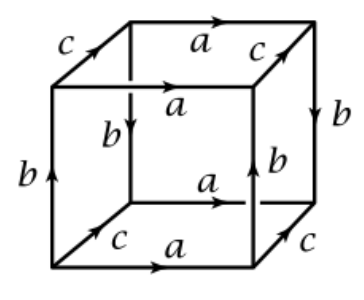
\includegraphics[scale=0.4]{prod1.png}
		\caption{Fundamental cube with CW-structure for $K\times\S^1$}
		\label{fig:prod}
	\end{figure}
	Here we denote $2$-simplices such that their boundary in $I^3$ does not contain their nominal letter in lowercase, e.g. $A$ is only bounded by copies of simplices $b$ and $c$ before identification.
	The obtained chain complex is now
	\[
	0 \xrightarrow{} \Z(V) \xrightarrow{\partial_3} \Z(A, B, C) \xrightarrow{\partial_2} \Z(a, b, c) \xrightarrow{\partial_1} \Z(p) \to 0.
	\]
	Again the map $\partial_1$ is clearly $0$ on all $1$-cycles, so we get
	\[
	\partial_1 = \begin{bmatrix}
	0 & 0 & 0
	\end{bmatrix},
	\]
	giving us
	\[
	H_0(K\times\S^1) = \Z(p)
	\]
	in the process.
	We now need to calculate the map $\partial_2$, which we will do using the cellular boundary formula
	\[
	\partial_2 E_i = \Sigma_j d_{ij}e_j
	\]
	where $E_i$ is one of the generating $2$-cycles and $d_{ij}$ are degrees defined as
	\[
	d_{ij} = \deg \Delta_{E_i,e_j} = \deg (\partial E_i \to X^{(1)} \to X^{(1)}/(X^{(1)}\setminus\lbrace e_j \rbrace)).
	\]
	The first map in the degree parantheses is the natural CW-complex attaching map and the second one is the collapsing map (as in the tutorial session). It is clear now that since $B$ attaches with the word $aca^{-1}c^{-1}$, all the degrees for $e_j \in \lbrace a, b, c \rbrace$ are $0$ and likewise for $C$, which attaches with the word $aba^{-1}b^{-1}$. The only exception is the $2$-simplex $A$, where we have a turning identification (so rotation, not reflection as for the rest), that is, it attaches with the word $bcbc^{-1}$, making $\deg\Delta_{A, b} = 2$ and the rest still zero. This gives us $\partial_2 A = 2b$, giving us the matrix
	\[
	\partial_2 =
	\begin{bmatrix}
	0 & 0 & 0 \\
	2 & 0 & 0 \\
	0 & 0 & 0
	\end{bmatrix}
	\]
	Thus clearly $\ker\partial_2 = \Z(B, C)$ and $\im\partial_2 = \Z(2b)$, which similar to 1.1 gives us
	\[
	H_1(K \times\S^1) = \ker\partial_1 / \im\partial_2 \iso \Z(a, b, c)/\Z(2b) \iso \Z\oplus\Z\oplus\Z_2.
	\]
	To calculate the map $\partial_3$ we employ the same procedure as above, but as we only have one generator, we merely need to calculate $3$ degrees $\Delta_{V,A}$, $\Delta_{V,B}$ and $\Delta_{V,C}$. As in the tutorial session, collapsing everything but $A$ to a point gives us two spheres identified by reflection (we don't turn when identifying), the coefficient at $A$ is $0$ (degree is $1 - 1 = 0$). Same argument works for $B$. With $C$, however, we identify by turning, making a rotation in our identification, meaning the degree of $\Delta_{V,C}$ is now $1 + 1 = 2$. Our matrix in this case is then
	\[
	\partial_3 = 
	\begin{bmatrix}
	0 \\ 0 \\ 2
	\end{bmatrix}
	\]
	which clearly gives is $\ker\partial_3 = 0$ and $\im\partial_3 = \Z(2C)$. The second homology group is now
	\[
	H_2(K\times\S^1) = \ker\partial_2 / \im\partial_3 \iso \Z \oplus \Z_2
	\]
	and the third homology group is
	\[
	H_3(K\times\S^1) = \ker\partial_3 = 0
	\]
	as expected.
	
	\item Lastly, we are computing the relative homology groups $H_n(K \times \S^1, \lbrace p, q \rbrace \times \S^1)$ for two different points $p, q \in K$. Recall the long exact sequence for homology of a pair $(X, A)$ is as follows
	\[
	\cdots \xrightarrow{\partial_*} H_n(A) \xrightarrow{i_*} H_n(X) \xrightarrow{q_*} H_n(X, A) \xrightarrow{\partial_*} H_{n-1}(A) \xrightarrow{} \cdots
	\]
	This sequence is non-trivial only for $n \leq 3$. We can do this from left to right or from right to left, we pick the former. For legibility's sake we will write only parts of the sequence at each step as it would otherwise span multiple lines. We also denote $X = K \times \S^1$ and $A = \lbrace p, q \rbrace \times \S^1$ to preserve form above. We start at $n = 3$ and get
	\[
	\cdots \xrightarrow{} 0 \xrightarrow{} 0 \xrightarrow{} H_3(X, A) \xrightarrow{} H_2(A) \xrightarrow{}\cdots
	\]
	but since $A$ is a manifold of dimension $1$, its second homology group is trivial and consequently
	\[
	H_3(X, A) = 0.
	\]
	We continue at $n=2$ and get
	\[
	0 \xrightarrow{} \Z \oplus \Z_2 \xrightarrow{} H_2(X, A) \xrightarrow{\partial_*} \Z\oplus\Z \xrightarrow{i_*} \Z\oplus\Z\oplus\Z_2 \xrightarrow{}\cdots
	\]
	Let $a, b$ be the generators of the free abelian group of $H_1(A) \iso \Z\oplus\Z$ (geometrically represented as the two distinct loops). Since $X$ and $K$ are connected and hence path connected, there exists a homotopy between the paths $i\circ a$ and $i\circ b$. By homotopy invariance in homology we get $i_*(a) = i_*(b)$ (in the sense of homology classes). Therefore one whole isomorphic copy of $\Z$ maps to $0$ with $i_*$ and we get $\ker i_* \iso \Z$. By exactness we have $\ker i_* = \im\partial_*$, therefore the following is an exact sequence
	\[
	0 \xrightarrow{} \Z\oplus\Z_2 \xrightarrow{} H_2(X, A) \xrightarrow{} \Z \xrightarrow{} 0
	\]
	Since the group on the right is a free group, by the splitting lemma the above short exact sequence splits, giving us the second relative homology group
	\[
	H_2(X, A) \iso \Z\oplus\Z\oplus\Z_2.
	\]
	We progress further to the right to $n=1$ and through the cokernel derive the following short exact sequence
	\[
	0 \xrightarrow{} \coker i_* \xrightarrow{} H_1(X, A) \xrightarrow{} \ker i_* \xrightarrow{} 0.
	\]
	We calculate
	\[
	\coker i_* = H_1(X)/\im i_* \iso \Z\oplus\Z\oplus\Z_2 / \Z \iso \Z\oplus\Z_2,
	\]
	and by exactness $\ker i_* = \im\partial_* \iso \Z$. The calculated sequence is now
	\[
	0 \xrightarrow{} \Z\oplus\Z_2 \xrightarrow{} H_1(X, A) \xrightarrow{} \Z \xrightarrow{} 0.
	\]
	By the same argument as above, the above short exact sequence splits and we again get
	\[
	H_1(X, A) \iso \Z\oplus\Z\oplus\Z_2.
	\]
	For the last group we again calculate taking exactness into account along the way
	\[
	H_0(X, A) \iso \im q_* \iso H_0(X)/\ker q_* \iso H_0(X)/\im i_* \iso \Z/\Z \iso 0
	\]
	which concludes the exercise.
\end{enumerate}

\underline{\textbf{Ex. 2:}}
Let $p \colon P \to X$ be a $2$-sheeted covering space over $X$.
\begin{enumerate}
	\item Consider the exact sequence
	\[
	0 \xrightarrow{} C_n(X;\Z_2) \xrightarrow{\tau} C_n(P; \Z_2) \xrightarrow{p_\#} C_n(X; Z_2) \xrightarrow{} 0.
	\]
	Here $\tau$ is given by $\tau(\sigma) = \overline{\sigma_1} + \overline{\sigma_2}$ where $\overline{\sigma_1}$ and $\overline{\sigma_2}$ are the two distinct lifts of simplex $\sigma\colon \Delta^n \to X$.
	
	Firstly, we need to show that the above sequence is exact for all $n \geq 0$.
	Clearly the map $p_\#$ is surjective, since $p$ is a covering projection. It is also easy to see that $\tau$ is injective, because the two lifts are by assumption distinct and hence do not sum into $0$ (note the $\Z_2$ coefficients). The only nontrivial part is the middle of the sequence. We're proving $\im\tau = \ker p_\#$. Inclusion from left to right follows easily, since $p_\#\tau(\sigma) = p_\#(\overline{\sigma_1} + \overline{\sigma_2}) = p_\#(\overline{\sigma_1}) + p_\#(\overline{\sigma_2}) = \sigma + \sigma = 0$ in $\Z_2$ coefficients. To prove the reverse inclusion, let $p_\#(\sigma) = p\circ\sigma = 0 \in C_n(X; \Z_2)$. We can now take the unique lift of $p\circ\sigma$, denoted by $\gamma = \overline{p\circ\sigma}$, which must of course be $0$. Then $\gamma$ must already be of the form $\tau(p\circ\sigma) \in \im\tau$ (again note the $\Z_2$ coefficients).
	
	Secondly, we want to show that the above exact sequences (for $n \geq 0$) form a short exact sequence of chain complexes. Since $\tau$ and $p_\#$ are already homomorphisms by definition, we only need to prove that they are indeed chain maps. In simpler terms, in the below diagram both squares must commute
	
	\adjustbox{scale=1, center}{
		\begin{tikzcd}
			0 \arrow[r] & C_n(X;\Z_2) \arrow[d,"\partial"] \arrow[r, "\tau"] &C_n(P;\Z_2) \arrow[d,"\partial"] \arrow[r, "p_\#"] &C_n(X; \Z_2) \arrow[d,"\partial"] \arrow[r]& 0 \\
			0 \arrow[r] & C_{n-1}(X;\Z_2) \arrow[r, "\tau"] &C_{n-1}(P;\Z_2) \arrow[r, "p_\#"] &C_{n-1}(X; \Z_2) \arrow[r]& 0
		\end{tikzcd}
	}
	Equation $\partial\circ p_\# = p_\# \circ \partial$ holds by definition of $p_\#$ as it is naturally defined by precomposition, that is, $p_\#(\sigma) = p \circ \sigma$.
	To prove $\partial \circ \tau = \tau \circ \partial$ take arbitrary $\sigma \in C_n(X;\Z_2)$. It suffices to prove that the boundary of a lift is a lift of the boundary, that is $\partial\overline{\sigma_i} = \overline{\partial\sigma_i}$. Indeed, by definition of the boundary map
	\[
	\partial\overline{\sigma_i} = \Sigma_j (-1)^j \overline{\sigma_i} \circ \phi_j = \Sigma_j \overline{\sigma_i} \circ \phi_j = \Sigma_j(\overline{\sigma\circ\phi_j})_i = (\overline{\partial\sigma})_i
	\]
	where $\phi_j$ gives us the $j$-th face of the simplex.
	Here we could remove the negative signs since we have $\Z_2$ coefficients. We also justify the third equality by observing that the point that determines the lift is arbitrary as long as it is in $\im(\overline{\partial\sigma_i}) \cap p^{-1}(\im(\sigma\circ\phi_j))$, since we must be able to map the lift back down.
	
	\item We now want to derive the associated long exact sequence and describe the connecting homomorphism on the level of chains.
	
	As in the case of homology of pair, using the snake lemma on the above exact sequence of chains we obtain
	\[
	\cdots \xrightarrow{\partial_*} H_n(X;\Z_2) \xrightarrow{\tau_*} H_n(P;\Z_2) \xrightarrow{p_*} H_n(X; \Z_2) \xrightarrow{\partial_*} H_{n-1}(X; \Z_2) \xrightarrow{} \cdots
	\]
	To describe the connecting homomorphism $\partial_*$ on the level of chains, we must take a cycle $\sigma \in C_n(X;\Z_2)$ and decompose it into simplices (recall, $C_n$ is an abelian group and as such a $\Z$-module). So let us write $\sigma = \Sigma_i \gamma_i$ where $\gamma_i$ are some generating simplices of dimension $n$. Note here that $\sigma$ is as a cycle a representative of some homology class usually denoted by $[\sigma] \in H_n(X; \Z_2)$. Since we have a covering space, let us try to observe what happens, when we try and lift this cycle $\sigma$, lift naturally meaning that $p_\#\overline{\sigma} = \sigma$ holds. Since $P$ is a $2$-sheeted covering space by assumption, every generating chain has two distinct lifts. Clearly when we lift the cycle $\sigma = \Sigma_i \gamma_i$, we lift the generating chains as well. However, as there are two possible lifts for any $\gamma_i$, let $\delta_i$ denote the index of the lift for $\gamma_i$ with respect to the lift of $\sigma$. In summation
	\[
	\overline{\sigma} = \Sigma_i (\overline{\gamma_i})_{\delta_i}.
	\]
	Here lifts of $\gamma_i$ are well defined by the covering space map lifting property as described in the diagram below
	
	\adjustbox{scale=1, center}{
		\begin{tikzcd}
			& P \arrow[d, "p"] \\
			\Delta^n \arrow[r, "\gamma_i"]\arrow[ru, "\overline{\gamma_i}_{1,2}"] & X
		\end{tikzcd}
	}
	Note that the lift of a cycle is in general not a cycle, but merely a chain.
	When we calculate the boundary of such a lift we get (taking into account similarities with 2.1)
	\[
	\partial\overline{\sigma} = \Sigma_i\partial(\overline{\gamma_i})_{\delta_i} = \Sigma_i (\overline{\partial\gamma_i})_{\delta_i}
	\]
	Since $\sigma$ is a cycle, by definition $\partial\sigma = 0$ holds, but the same cannot be said for the lift $\overline{\sigma}$. Recall now the diagram from 2.1 proving that we have a short exact sequence of chain complexes. By commutiativity of the right square we have $\partial\circ p_\# = p_\# \circ \partial$, therefore $p_\#(\partial\overline{\sigma}) = \partial(p_\#(\overline{\sigma})) = \partial(\sigma) = 0$ and hence $\partial\overline{\sigma} \in \ker p_\#$. In other words, for every $\gamma_i$ there exists a chain one dimension lower $\epsilon_i \in C_{n-1}(X;\Z_2)$ such that by exactness the following holds
	\[
	\tau(\epsilon_i) = (\overline{\epsilon_i})_1 + (\overline{\epsilon_i})_2 = (\overline{\partial\gamma_i})_{\delta_i}.
	\]
	In homology, it now follows that
	\[
	\partial_*[\sigma] = \Sigma_i[\epsilon_i].
	\]
	This is nothing surprising, as $\partial_*$ was induced by the connecting morphism $\partial$. On the level of generating chains we see that this is just the boundary morphism.
	
	Consider now the figure from the instruction set and let us calculate $\partial c_1$ and $\partial c_2$, where $c_1 = [01] + [02] + [12]$ and $c_2 = [012] + [013] + [023] + [123]$ are given $1$- and $2$- cycles respectively with $\Z_2$ coefficients.
	
	For $c_1$ we calculate (all with pluses since we have $\Z_2$ coefficients)
	\begin{align*}
	\partial_* c_1 &= \partial\overline{c_1} = \overline{\partial[01]}_{\delta_1} + \overline{\partial[02]}_{\delta_2} + \overline{\partial[12]}_{\delta_3} \\
	&= \overline{[0]}_{\delta_1} + \overline{[1]}_{\delta_1} + \overline{[0]}_{\delta_2} + \overline{[2]}_{\delta_2} + \overline{[1]}_{\delta_3} + \overline{[2]}_{\delta_3}
	\end{align*}
	Now recall that since $P$ is a $2$-sheeted covering space, $\delta_i \in \lbrace 1, 2 \rbrace$, but $i \in \lbrace 1, 2, 3 \rbrace$. By the pidgeonhole principle, at least two of the indices $\delta_i$ must be the same. We analyse case by case
	\begin{itemize}
		\item Suppose $\delta_1 = \delta_2 = \delta_3$, which is the same as saying that we have lifted $c_1$ to a cycle. Indeed all $0$-simplices cancel and we get $\partial_* c_1 = 0$.
		\item Suppose $\delta_1 = \delta_2 \neq \delta_3$. Then
		\[
		\partial_* c_1 = \overline{[1]}_{\delta_1} + \overline{[2]}_{\delta_1} + \overline{[1]}_{\delta_2} + \overline{[2]}_{\delta_2}
		\]
		However, this are pricesely both of the lifts for $\partial [12]$. On the level of chains, we get that $\partial c_1 = [1] + [2] = \partial[12]$, but on the level of homology, since we got both lifts, this is the same as the previous possibility, that is, trivial.
		\item We do similarly for other possibilities (since there can only be one different index at a time).
	\end{itemize}
	 
	 The calculation for $c_2$ will be the same, but there will be more non-analogous possibilities. We calculate
	 \begin{align*}
	 \partial_* c_2 = \partial\overline{c_2} &= \overline{[12]}_{\delta_1} + \overline{[02]}_{\delta_1} + \overline{[01]}_{\delta_1} + \overline{[13]}_{\delta_2} + \overline{[03]}_{\delta_2} + \overline{[01]}_{\delta_2} \\
	 &+ \overline{[23]}_{\delta_3} + \overline{[03]}_{\delta_3} + \overline{[02]}_{\delta_3} + \overline{[23]}_{\delta_4} + \overline{[13]}_{\delta_4} + \overline{[12]}_{\delta_4}
	 \end{align*}
	 Now we have $i \in \lbrace 1, 2, 3, 4 \rbrace$, so again by pidgeonhole principle, at least two indices $\delta_i$ must be the same. We analyse case by case
	 \begin{itemize}
	 	\item Suppose all indices are the same. Then as before all $1$-simplices cancel out (since they all appear exactly twice with in general possibly different indices) and we get $\partial_* c_2 = 0$.
	 	\item Suppose one of the indices is different, without loss of generality let it be the last index $\delta_4$. Then lifts of simplices $[23]$, $[13]$ and $[12]$ are the only ones that do not cancel out with their counterparts and we get
	 	\[
	 	\partial\overline{c_2} =\overline{[23]}_{\delta_1} + \overline{[13]}_{\delta_1} + \overline{[12]}_{\delta_1} + \overline{[23]}_{\delta_4} + \overline{[13]}_{\delta_4} + \overline{[12]}_{\delta_4}
	 	\]
	 	already inputing $\delta_1 = \delta_2 = \delta_3$. Again we have both lifts of certain simplices present, therefore $\partial_* c_2 = [23] + [13] + [12] = \partial [123]$, while on the level of homology this is again trivial. Similarly for other possibilities where only one index is different.
	 	\item Suppose finally that two of the indices are different from the other two, without loss of generality $\delta_1 = \delta_2$ and $\delta_3 = \delta_4$. Here we see that the lifts of simplices $[01]$ and $[23]$ cancel and the rest persist, but again with both lifts, so we get $\partial_* c_2 = [12] + [02] + [13] + [03]$ (in the order they appear above). We see that this combination clearly forms a $1$-cycle with $\Z_2$ coefficients (say $1 \to 2 \to 0 \to 3 \to 1$). This is also equal to the trivial homology class on the level of homology, since
	 	\[
	 	\partial_* c_2 = [12] + [02] + [13] + [03] = [12] + [02] + [01] + [01] + [13] + [03] = \partial [012] + \partial [013]
	 	\]
	 	Similarly for the other possibilities with such an index partition.
	\end{itemize}
 	
 	\item To conclude the exercise let $n \geq 2$ and let us calculate $H_k(\R\P^n; \Z_2)$ using the above long exact sequence for the covering projection $p\colon \S^n \to \R\P^n$.
 	
 	Firstly, recall that $H_k(\S^n; \Z_2) \neq 0$ precisely when $k \neq 0, n$, in which case it is equal to $\Z_2$. Secondly, the instructions make sense, since $\S^n$ is indeed a $2$-sheeted cover of $\R\P^n$. The needed long exact sequence is as follows
 	\[
 	\cdots \xrightarrow{\partial_*} H_k(\R\P^n; \Z_2) \xrightarrow{\tau_*} H_k(\S^n; \Z_2) \xrightarrow{p_*} H_k(\R\P^n; \Z_2) \xrightarrow{\partial_*} H_{k-1}(\R\P^n; \Z_2) \xrightarrow{} \cdots
 	\]
 	To deal with the obvious, since $\R\P^n$ is connected and therefore path connected, $H_0(\R\P^n; \Z_2) \iso \Z_2$. Now that we have this out of the way, for $k < n$ we get short exact sequences of the form
 	\[
 	0 \xrightarrow{} H_k(\R\P^n; \Z_2) \xrightarrow{} H_{k-1}(\R\P^n; \Z_2) \xrightarrow{} 0
 	\]
 	just by taking into account that $H_k(\S^n; \Z_2) = 0$ for $0 < k < n$. Therefore $H_k(\R\P^n; \Z_2) \iso \Z_2$ for all $k < n$.
 	For $k = n$ we get the sequence
 	\[
 	0 \xrightarrow{} H_n(\R\P^n; \Z_2) \xrightarrow{} \Z_2 \xrightarrow{} H_n(\R\P^n; \Z_2) \xrightarrow{} \Z_2 \xrightarrow{} 0
 	\]
 	which immediately implies $H_n(\R\P^n ; \Z_2) = \Z_2$, since the only other possibility by the left part of the sequence (injectivity of $\tau_*$) is $H_n (\R\P^n ; \Z_2) = 0$, which would by exactness imply $\Z_2 = 0$, leading to a contradiction. All higher homology groups are of course clearly trivial. In summation
 	\[
 	H_k(\R\P^n) = \begin{cases}
 	\Z_2 \text{ if $k \leq n$}\\
 	0 \text{ otherwise}
 	\end{cases}
 	\]
\end{enumerate}

\underline{\textbf{Ex. 3:}}
Let $X = U_0 \cup U_1 \cup \cdots \cup U_N$ where $U_i \subseteq X$ are open subsets. Denote by $U_{ij} = U_i \cap U_j$ the intersections and assume that all triple and higher intersections are empty. Consider the following sequence
\[
0 \xrightarrow{} \bigoplus_{i<j}C_n(U_{ij}) \xrightarrow{\Phi} \bigoplus_{i}C_n(U_i) \xrightarrow{\Pi} C_n(U_0 + U_1 + \cdots + U_N) \xrightarrow{} 0
\]
where the maps $\Phi, \Pi$ are given by
\[
\Phi(0,\dots, 0, \alpha_{ij}, 0, \dots, 0) = (0, \dots, 0, \underbrace{\alpha_{ij}}_i, 0, \dots, 0, \underbrace{-\alpha_{ij}}_j, 0, \dots, 0)
\]
and
\[
\Pi(\alpha_0, \dots, \alpha_N) = \alpha_0 + \cdots + \alpha_N.
\]
\begin{enumerate}
	\item Let us first show that the above sequence is exact for all $n\geq 0$ and that these short exact sequences form a short exact sequence of chain complexes. Then we will naturally derive the associated long exact sequence.
	
	First note, that $C_n(U_0 + U_1 + \cdots + U_N)$ is precisely the free abelian group generated by all generators of $C_n(U_i)$ for $0 \leq i \leq N$. We immediately see that $\Phi$ is injective and $\Pi$ is surjective by their respective definitions, so what remains to show for exactness is $\ker\Pi = \im\Phi$. First we verify that their composition is trivial. Indeed
	\[
	\Pi\Phi(0,\dots,0,\alpha_{ij}, 0, \dots, 0) = \Pi(0, \dots, 0, \alpha_{ij}, 0, \dots, 0, -\alpha_{ij}, 0, \dots, 0) = \alpha_{ij} - \alpha_{ij} = 0.
	\]
	For the reverse inclusion take $(\alpha_0, \dots, \alpha_N) \in \ker\Pi$. This is equivalent to the sum of $\alpha_i$'s being equal to $0$. Also note that we need only verify our claim on the generators, that is, $\alpha_i$ being simplices, as we are dealing with homomorphisms (which are defined on generators).
	We want to prove that there exist simplices $\alpha_{ij}$ such that they together are mapped to our element. We have to somehow move to the intersections. For that reason define $\alpha_i|^{U_i\cap U_j} \in C_n(U_i \cap U_j)$ as the restriction of $\alpha_i$'s codomain $U_i$ to $U_i \cap U_j$. This restriction is continuous since the sets $U_i$ (and of course their intersecions) are open. Note that this restriction can be non-trivial, but in any case from our assumption about higher intersections we get that $\im(\alpha_k|^{U_k \cap U_l}) \cap U_i \cap U_j = \emptyset$ for all $i, j, k$ pairwise different. We can now partition the codomain $U_i$ of $\alpha_i$ even more into disjoint set as follows
	\[
	U_i = (U_i \setminus \cup_{i \neq j} U_j) \bigcup (\cup_{i \neq j}(U_i \cap U_j))
	\]
	and therefore
	\[
	\alpha_i = \alpha_i|^{U_i \setminus \cup_{i \neq j}U_j} + \Sigma_{i \neq j}\alpha_i|^{U_i \cap U_j}.
	\]
	However, since the sum of all $\alpha_i$ is zero, then so is the sum of restrictions $\alpha_i|^{U_i \setminus \cup_{i \neq j}U_j}$ to now disjoint codomains. It is now clear that $\alpha_i|^{U_i \setminus \cup_{i \neq j}U_j} = 0$ for all $0 \leq i \leq N$. Therefore $\Phi(\oplus_{i<j}\alpha_{ij}) = (\alpha_0,\dots, \alpha_N)$, proving the statement.
	
	As in exercise 2, to prove that the sequences give rise to a short exact sequence of chain complexes, we need to only prove the commutativity of the following diagram
	
	\adjustbox{scale=1, center}{
		\begin{tikzcd}
			0 \arrow[r] & \bigoplus_{i<j} C_n(U_{ij}) \arrow[d,"\partial"] \arrow[r, "\Phi"] & \bigoplus_{i} C_n(U_i) \arrow[d,"\partial"] \arrow[r, "\Pi"] &C_n(U_0 + \cdots + U_N) \arrow[d,"\partial"] \arrow[r]& 0 \\
			0 \arrow[r] & \bigoplus_{i<j} C_{n-1}(U_{ij}) \arrow[r, "\Phi"] & \bigoplus_{i} C_{n-1}(U_i) \arrow[r, "\Pi"] &C_{n-1}(U_0 + \cdots + U_N) \arrow[r]& 0
		\end{tikzcd}
	}

	The calculation here is easier than in exercise 2. We calculate directly
	\begin{align*}
	\Phi(\partial(0,\dots,0,\alpha_{ij},0,\dots,0)) &= \Phi(0,\dots,0,\partial\alpha_{ij},0,\dots,0) = (0,\dots,0,\partial\alpha_{ij}, 0,\dots,0,-\partial\alpha_{ij}, 0,\dots,0) \\
	\partial(\Phi(0,\dots,0,\alpha_{ij},0,\dots,0)) &= \partial(0,\dots,0,\alpha_{ij}, 0,\dots,0,-\alpha_{ij}, 0,\dots,0) \\
	&= (0,\dots,0,\partial\alpha_{ij}, 0,\dots,0,-\partial\alpha_{ij}, 0,\dots,0)
	\end{align*}
	which proves the commutativity of the left square, and
	\begin{align*}
	\Pi(\partial(\alpha_0, \dots, \alpha_N)) &= \Pi(\partial\alpha_0, \dots, \partial\alpha_N) = \partial\alpha_0 + \cdots + \partial\alpha_N \\
	\partial(\Pi(\alpha_0, \dots, \alpha_N)) &= \partial(\alpha_0 + \cdots + \alpha_N) = \partial\alpha_0 + \cdots + \partial\alpha_N
	\end{align*}
	which finally shows, that we have a short exact sequence of chain complexes. Same as before, by using snake lemma, we get the associated long exact sequence
	\[
	\cdots \xrightarrow{\partial_*} \bigoplus_{i<j}H_n(U_{ij}) \xrightarrow{\Phi_*} \bigoplus_{i}H_n(U_i) \xrightarrow{\Pi_*} H_n(U_0 + \cdots + H_N) \xrightarrow{\partial_*} \bigoplus_{i<j}H_{n-1}(U_{ij}) \xrightarrow{} \cdots
	\]
	Why can we write pluses like above? Observe that this is precisely the generalized Mayer-Vietoris sequence. In the proof of the theorem we used the fact that $H_*$ is an additive functor and it's the same fact we use here to justify the above associated sequence.
	
	\item We will now use the above associated long exact sequence to compute the homology of the circle $\S^1$, partitioned with $4$ open arcs $U_0, U_1, U_2, U_3$ as shown in the figure in the instruction set.
	
	The first thing we notice is that all intersections of sets $U_{ij}$ and the sets $U_i$ themselves are homeomorphic to intervals or unions of intervals, which are homotopy equivalent to points. Secondly, we're calculating $H_n(\S^1)$, which does not appear to be in our sequence. However, as we have an inclusion $C_n(U_0 + \cdots + U_N) \to C_n(\S^1)$, this inclusion induces an isomorphism of homology groups $H_n(U_0 + \cdots + U_N) \to H_n(\S^1)$ as in the regular Mayer-Vietoris sequence. Taking into account our first observation, all homology groups $H_n(\S^1)$ for $n\geq 2$ are trivial, as all groups around them in the sequence are trivial, so our sequence transforms into
	\[
	0 \xrightarrow{} H_1(\S^1) \xrightarrow{} \bigoplus_{i<j}H_0(U_{ij}) \xrightarrow{} \bigoplus_{i}H_0(U_i) \xrightarrow{} H_0(\S^1) \xrightarrow{} 0
	\]
	As there are four intersection parts and four partition arcs,
	the sequence now looks like
	\[
	0 \xrightarrow{} H_1(\S^1) \xrightarrow{\partial_*} \Z^4 \xrightarrow{\Phi_*} \Z^4 \xrightarrow{\Pi_*} H_0(\S^1) \xrightarrow{} 0
	\]
	where $\Z^4$ denotes $\Z\oplus\Z\oplus\Z\oplus\Z$ for brevity.
	
	But recall now that $\S^1$ is a path connected space, so $H_0(\S^1) \iso \Z$. Focusing on the map $\Phi_*$ we separate the above sequence by forcing in $\im\Phi_*$ to get two short exact sequences
	\[
	0 \xrightarrow{} \im\Phi_* \Z^4 \xrightarrow{} \Z \xrightarrow{} 0
	\]
	and
	\[
	0 \xrightarrow{} H_1(\S^1) \xrightarrow{} \Z^4 \xrightarrow{} \im\Phi_* \xrightarrow{} 0.
	\]
	As before, since $\Z$ is a free group, the first sequence splits and implies $\im\Phi_* \iso \Z^3$. Since $\Z^3$ is also a free group, the second sequence splits as well and implies $H_1(\S^1) \iso \Z$.
	
%	We progress from left to right. By exactness, $\partial_*$ is an injective homomorphism and is therefore isomorphic to its image. Hence $H_1(\S^1) \iso \im\partial_* \iso \ker\Phi_*$ where the last isomorphism follows again by exactness. So take a cycle $(\alpha_{ij})_{i<j} \in \ker\Phi_* \subseteq \bigoplus_{i<j}H_0(U_{ij})$. Since our indices go only to $3$, we see that $(\alpha_{ij})_{i<j} = (\alpha_{01}, \alpha_{03}, \alpha_{12}, \alpha_{23})$ skipping empty intersections. In detail we now have
%	\[
%	0 = \Phi_* (\alpha_{01}, \alpha_{03}, \alpha_{12}, \alpha_{23}) = (\alpha_{01} + \alpha_{03}, -\alpha_{01} + \alpha_{12}, -\alpha_{12}+ \alpha_{23}, -\alpha_{03} - \alpha_{23})
%	\]
%	Writing out equations we get $\alpha_{03} = -\alpha_{01}$, $\alpha_{12} = \alpha_{01}$ and $\alpha_{23} = \alpha_{12} = \alpha_{01}$, so $(\alpha_{ij})_{i<j} = (\alpha_{01}, -\alpha_{01}, \alpha_{01}, \alpha_{01})$, so $\ker\Phi_*$ is $1$-dimensional and thus isomorphic to $\Z$. This proves $H_1(\S^1) \iso \Z$ as previously known.
%	
%	Further to the right, again by exactness we know $H_0(\S^1) \iso \im \Pi_*$. By the first isomorphism theorem it must hold that $\im\Pi_* \iso \bigoplus_{i}H_0(U_i)/\ker\Pi_*$. Similarly to above we show that $\ker\Pi_*$ is indeed $3$-dimensional and therefore isomorphic to $\Z^3$, giving us the expected result $H_0(\S^1) \iso \Z$.
	
	 \item The last thing to do now is to use the associated long exact sequence above to compute the homology of $X = \S^1\vee\S^2$ by taking $U_0$, $U_1$ and $U_2$ as in the figure in the instruction set. For better intuition, $U_0$ is an arc, therefore homotopy equivalent to a point, $U_2$ is a hemisphere, so homeomorphic to a disc and therefore again homotopy equivant to a point. The set $U_1$ is a wedge of an arc and a hemisphere, which is again contractible and hence homotopy equvalent to a point. The interesting parts here are the intersections. The first intersection $U_0 \cap U_1$ is a disjoint union of two arcs/intervals, while $U_1 \cap U_2$ is a strip around $\S^2$ and therefore homotopy equivalent to $\S^1$.
	 
	 Clearly all homology groups for $n \geq 3$ are trivial, so we look at our sequence at $n=2$ and up to isomorphism in homology get
	 \[
	 0 \xrightarrow{} \bigoplus_{i<j}H_2(U_{ij}) \xrightarrow{} \bigoplus_{i}H_2(U_i) \xrightarrow{} H_2(X) \xrightarrow{} \bigoplus_{i<j}H_1(U_{ij}) \xrightarrow{} \bigoplus_{i}H_1(U_i) \xrightarrow{} \cdots
	 \]
	 We fill in known groups and our sequence transforms into
	 \[
	 0 \xrightarrow{} 0 \xrightarrow{} 0 \xrightarrow{} H_2(X) \xrightarrow{} \Z \xrightarrow{} 0
	 \]
	 By exactness $H_2(X) \iso \Z$. Further to the right we have
	 \[
	 0 \xrightarrow{} H_1(X) \xrightarrow{\partial_*} \bigoplus_{i<j}H_0(U_{ij}) \xrightarrow{\Phi_*} \bigoplus_{i} H_0(U_i) \xrightarrow{} H_0(X) \xrightarrow{} 0
	 \]
	 Again we use that $\S^1\vee\S^2$ is path connected, so $H_0(X) \iso 0$. Filling in the rest of known groups we get
	 \[
	 0 \xrightarrow{} H_1(X) \xrightarrow{\partial_*} \Z^2\oplus\Z \xrightarrow{\Phi_*} \Z^3 \xrightarrow{} \Z \xrightarrow{} 0
	 \]
	 where $\Z^2$ comes from the two disjoint intervals in $U_{01}$.
	 We again separate this sequence by forcing in $\im\Phi_*$ to get the following two exact sequences
	 \[
	 0 \xrightarrow{} \im\Phi_* \xrightarrow{} \Z^3 \xrightarrow{} \Z \xrightarrow{} 0
	 \]
	 and
	 \[
	 0 \xrightarrow{} H_1(X) \xrightarrow{} \Z^3 \im\Phi_* \xrightarrow{} 0.
	 \]
	 As in 3.2, since $\Z$is a free group, the first sequence splits implying $\im\Phi_* \iso \Z^2$, and again since $\Z^2$ is also a free group, the second sequence splits as well, giving us $H_1(X) \iso \Z$. This concludes the exercise as we have calculated all non-trivial homology groups of $\S^1\vee\S^2$.
%	 By exactness, $\partial_*$ is injective and $H_1(X) \iso \im\partial_* \iso \ker\Phi_*$. Similarly to 3.2 we take $(\alpha_{01}, \alpha_{12}) \in \ker\Phi_* \subseteq H_0(U_{01}) \oplus H_0(U_{12})$. Denote also $\alpha_{01} = (\alpha_{01}', \alpha_{01}'')$. We calculate
%	 \[
%	 0 = \Phi_*(\alpha_{01}, \alpha_{12}) = (\alpha_{01}' + \alpha_{01}'', -\alpha_{01}' -\alpha_{01}'' + \alpha_{12}, -\alpha_{12})
%	 \]
%	 giving us equations $\alpha_{12} = 0$ and $\alpha_{01}' = -\alpha_{01}''$. Hence $\ker\Phi_*$ is $1$-dimensional and isomorphic to $\Z$.
%	 
%	 
%	 With $\Pi_*$ we can easily calculate that $H_0(X) \iso \Z$, but we already know that as $X$ is path connected. This concludes the exercise for we have calculated all non-trivial homology groups of $\S^1\vee\S^2$.
\end{enumerate}
\end{document}

%% TEMPLATES
% lists
%\begin{enumerate}[label=(\alph*)]
% diagram
%\adjustbox{scale=1, center}{
%	\begin{tikzcd}
%		\R_n \arrow[d, "\varphi_n"] \arrow[r, "\Phi"] & \R_m \arrow[d, "\varphi_m"] \\
%		\R \arrow[r, "\widetilde{\Phi}"] & \R
%	\end{tikzcd}
%}
% figure
%\begin{figure}[h]
%	\centering
%	\includegraphics[scale=0.4]{fig}
%	\caption{caption}
%	\label{fig:label}
%\end{figure}
